\section{Exercise 1: Haar-like features and classification}

\subsection{Compute and visualize Haar-like features}

\ref{fig:integralim}

\ref{fig:mask1}

\ref{fig:mask2}

\ref{fig:featscatter}

\ref{fig:facesandnonfaceshighlighted}

\ref{fig:feattestscatter}

\ref{fig:testfaceshighlighted}

\begin{figure}[h!tb]
	\centering
		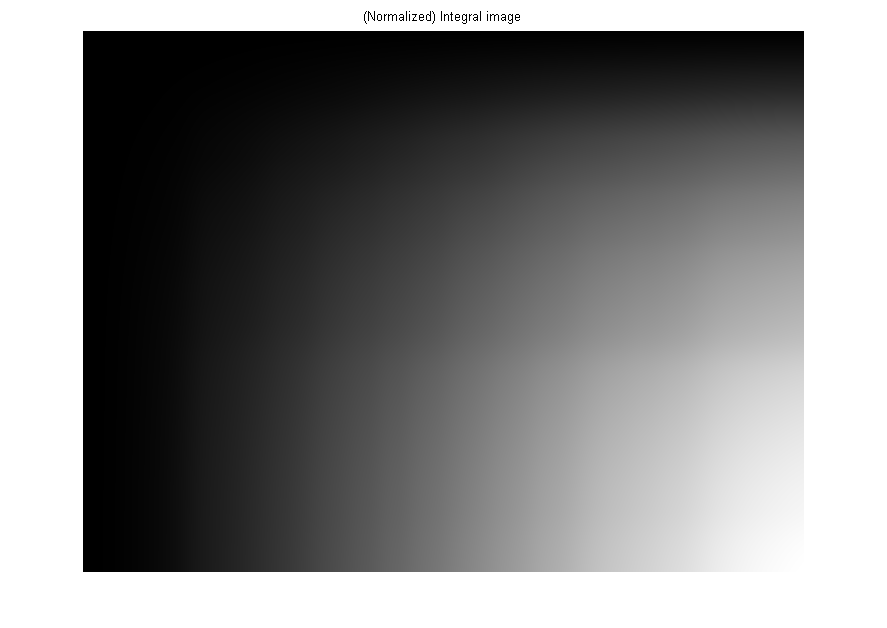
\includegraphics[width=\textwidth]{./img/ex1/integralim.png}
	\caption{Integral image}
	\label{fig:integralim}
\end{figure}

{\bfseries
Question 1:
\begin{itemize}
\item Explain the obtained 2-dimensional plot on the feature space.
\item Given this 2-dimensional plot, can we infer the defined Haar-like features are appropriate for face/non-face discrimination?
\end{itemize}}


\begin{figure}[h!tb]
	\centering
		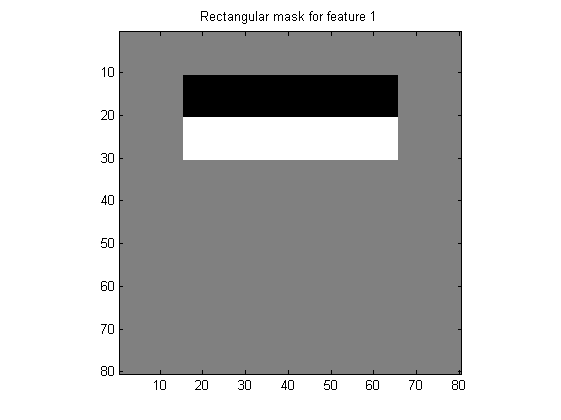
\includegraphics[width=\textwidth]{./img/ex1/mask1.png}
	\caption{Mask for computing the first feature}
	\label{fig:mask1}
\end{figure}

\begin{figure}[h!tb]
	\centering
		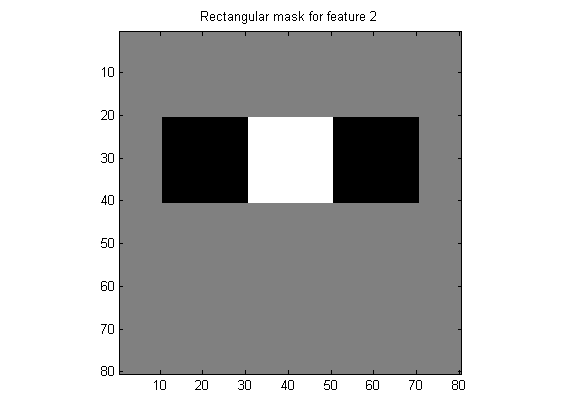
\includegraphics[width=\textwidth]{./img/ex1/mask2.png}
	\caption{Mask for computing the second feature}
	\label{fig:mask2}
\end{figure}

\begin{figure}[h!tb]
	\centering
		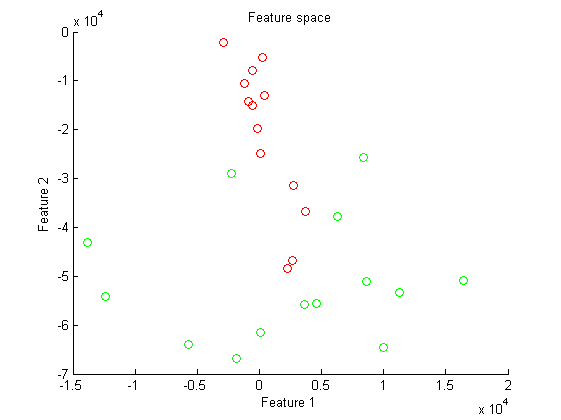
\includegraphics[width=\textwidth]{./img/ex1/featscatter.png}
	\caption{Scatter plot of the features for faces and non-faces}
	\label{fig:featscatter}
\end{figure}

\begin{figure}[h!tb]
	\centering
		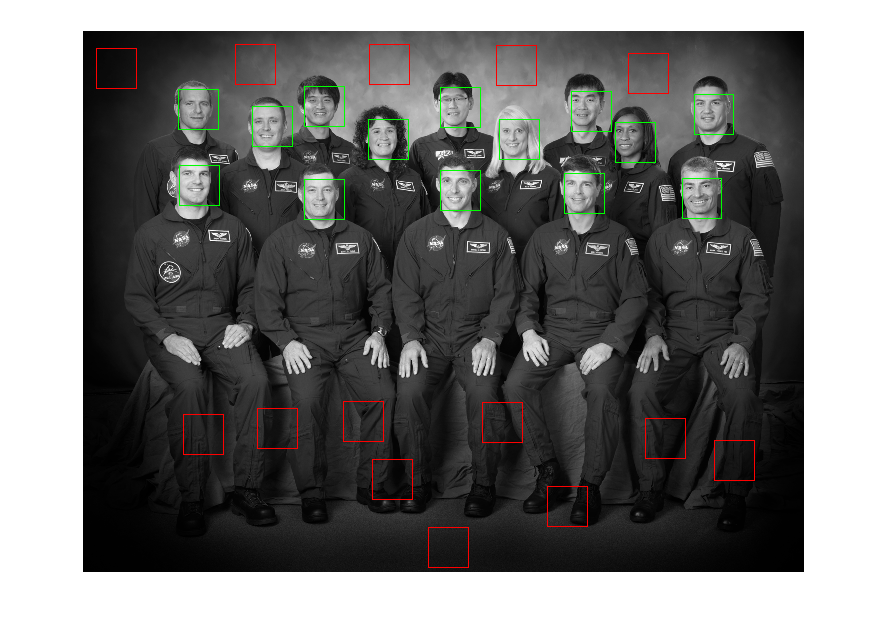
\includegraphics[width=\textwidth]{./img/ex1/facesandnonfaceshighlighted.png}
	\caption{Highlighted faces \& non-faces}
	\label{fig:facesandnonfaceshighlighted}
\end{figure}

\begin{figure}[h!tb]
	\centering
		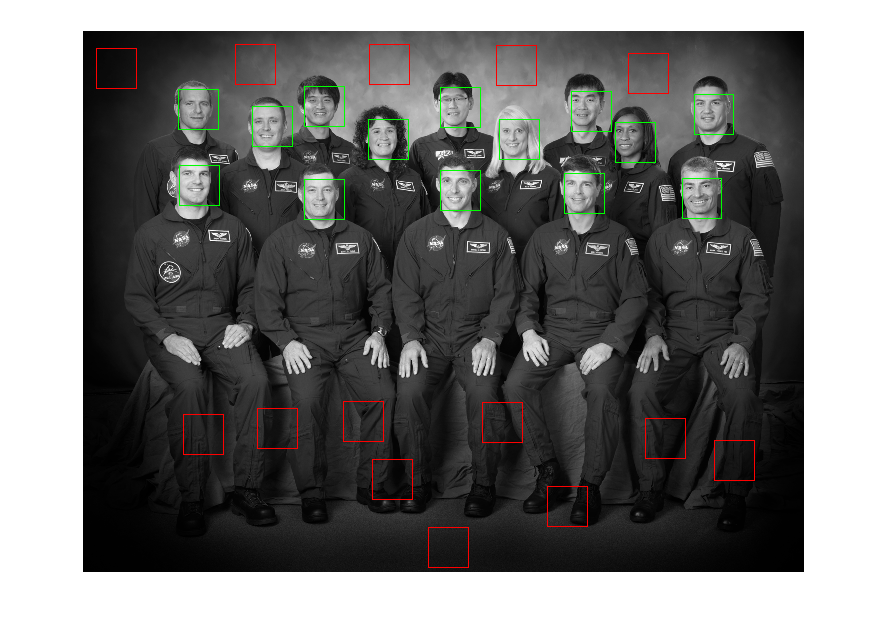
\includegraphics[width=\textwidth]{./img/ex1/facesandnonfaceshighlighted.png}
	\caption{Highlighted faces \& non-faces}
	\label{fig:facesandnonfaceshighlighted}
\end{figure}


\subsection{Classification in the feature space}

{\bfseries Question 2: \\Is the result good enough? Explain your response}

{\bfseries Question 3: \\What do you infer from the figure? Explain your response}

\begin{figure}[h!tb]
	\centering
		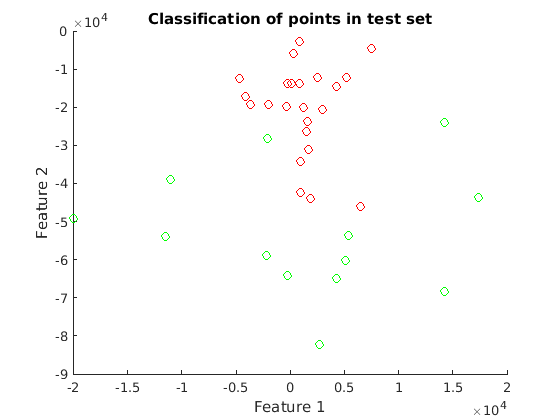
\includegraphics[width=\textwidth]{./img/ex1/feattestscatter.png}
	\caption{Highlighted faces \& non-faces (test set)}
	\label{fig:feattestscatter}
\end{figure}

\begin{figure}[h!tb]
	\centering
		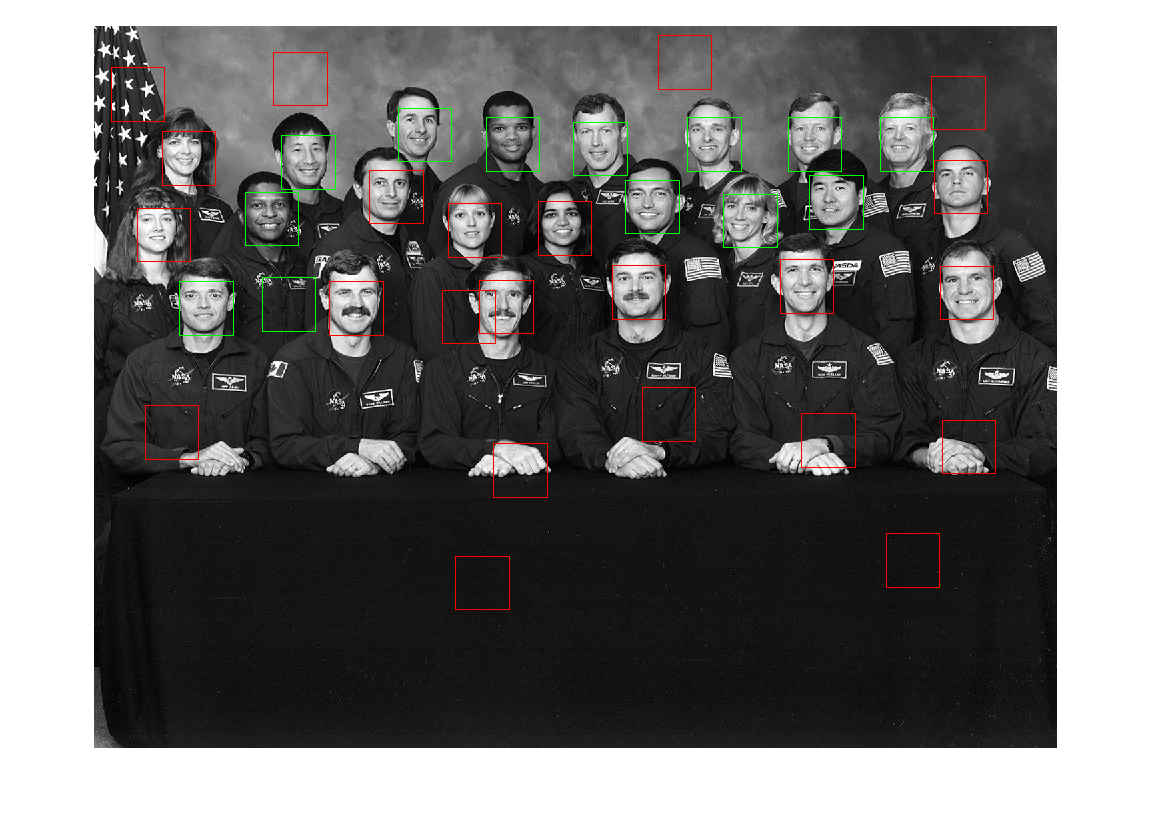
\includegraphics[width=\textwidth]{./img/ex1/testfaceshighlighted.png}
	\caption{Highlighted faces \& non-faces (test set)}
	\label{fig:testfaceshighlighted}
\end{figure}